Karo pabėgėliu mėnesinis skaičius pagal šalis\cite{refugees} buvo sutrauktas į bendrą per mėnesinį pasaulio babėgėlių skaičių 2003 - 2017 metais.
Žodžio „war“ skaičius per mėnesį buvo surinktas iš ABC naujienų portalo antraščių\cite{abcNews} tuo pačiu laikotarpiu.

\begin{figure}
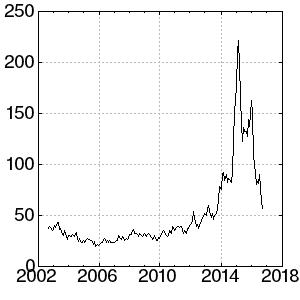
\includegraphics[scale=0.65]{../scripts/refugees_war/refugees.png}
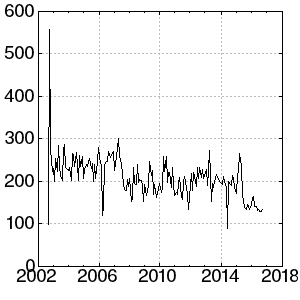
\includegraphics[scale=0.65]{../scripts/refugees_war/war.png}
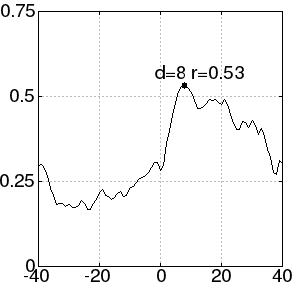
\includegraphics[scale=0.65]{../scripts/refugees_war/result.png}
    \caption{Grafikas kairėje: vidutinis mėnesinis karo pabėgėlių skaičius pasaulyje. Grafikas centre: mėnesinis „war“ skaičius ABC naujienų antraštėse. Grafikas dešinėje: signalų tarpusavio koreliacija}
\end{figure}

Nors tarp karo pabėgėlių ar žodžio „war“ dažnumo grafiko akivaizdaus ryšio nesimato,
poros koreliacijos funkcija rodo didžiausią signalų panašumą \( R_{fg}(t) = 0.53 \), kai \( t = 8 \).
